\chapter{Neuronavegation}
\label{sec:neuronavegador}

An introduction to neuronavigation theory was presented in section~\ref{sec:neuronavegador_intro}. Please read that section before using the features detailed below.

To enable the InVesalius neuronavigation mode, select the \textbf{Mode} tab in the main menu and then Navigation (Figure~\ref{fig:nav_menu_en}). A \textbf{Navigation System} tab will then display in the panel to the left of the main window, as shown in Figure~\ref{fig:nav_painel_en}.

\begin{figure}[!htb]
\centering
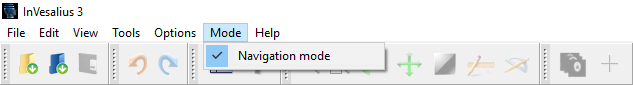
\includegraphics[scale=0.4]{../user_guide_figures/invesalius_screen/nav_menu_en.png}
\caption{Menu to enable neuronavigation mode.}
\label{fig:nav_menu_en}
\end{figure}

\begin{figure}[!htb]
\centering
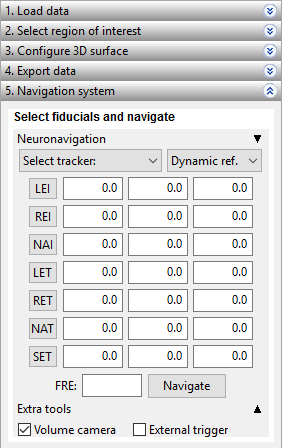
\includegraphics[scale=0.6]{../user_guide_figures/invesalius_screen/nav_painel_en.png}
\caption{Tab for navigation system.}
\label{fig:nav_painel_en}
\end{figure}

\section{Spatial trackers and reference mode}

Currently, InVesalius Navigator supports four spatial tracking devices from two manufacturers: the MicronTracker from ClaroNav (Toronto, Canada; Figure~\ref{fig:tracker_claron}) and Fastrak, Isotrak and Patriot from Polhemus (Colchester, United States; Figure~\ref{fig:tracker_polhemus}).

First, choose the tracker in the menu \textbf{Select tracker} (Figure~\ref{fig:nav_select_tracker}). The option \textbf{Debug tracker} allows the user to test the system even if there is no spatial tracker connected, instead simulating a spatial tracker by generating random coordinates.

\begin{figure}[!htb]
\centering
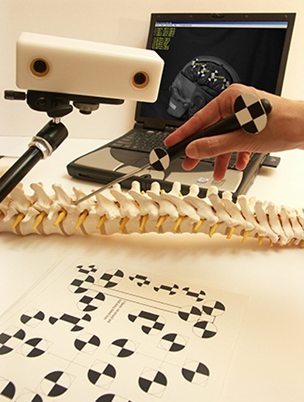
\includegraphics[scale=0.4]{../user_guide_figures/tracker_claron.png}
\caption{ClaroNav MicronTracker - www.claronav.com/microntracker/.}
\label{fig:tracker_claron}
\end{figure}

\begin{figure}[!htb]
\centering
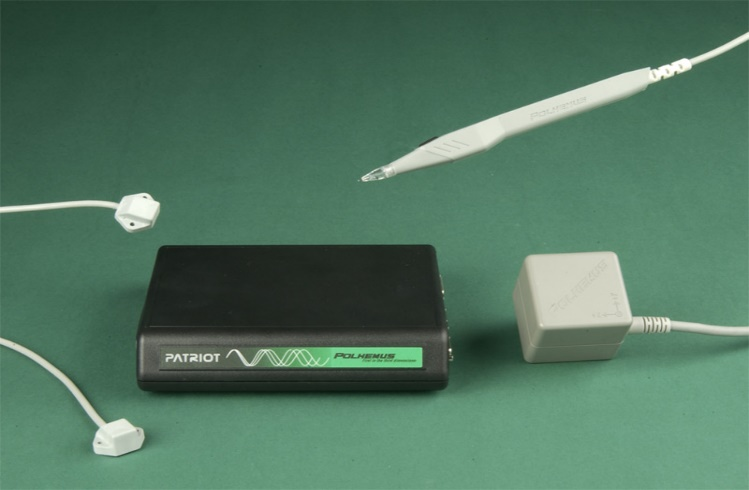
\includegraphics[scale=0.5]{../user_guide_figures/tracker_polhemus.jpg}
\caption{Polhemus Patriot tracker - http://polhemus.com/motion-tracking/overview/.}
\label{fig:tracker_polhemus}
\end{figure}

\begin{figure}[!htb]
\centering
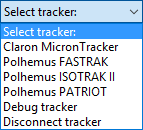
\includegraphics[scale=0.6]{../user_guide_figures/invesalius_screen/nav_select_tracker_en.png}
\caption{Menu to select tracking device.}
\label{fig:nav_select_tracker}
\end{figure}

There are two methods to perform the navigation: static and dynamic (Figure~\ref{fig:nav_menu_ref}). Static mode uses just one spatial tracker probe. In this mode, the subject's head must stay motionless after registration (for more info about coregistration see Section~\ref{sec:corregistro} probes: a reference probe must head (e.g. forehead). during the probe will detect and correct any 16.2). Dynamic mode uses multiple be attached to a static part of the neuronavigation process; the reference movements from the head.

\begin{figure}[!htb]
\centering
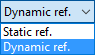
\includegraphics[scale=0.6]{../user_guide_figures/invesalius_screen/nav_menu_ref_en.png}
\caption{Menu to select reference mode.}
\label{fig:nav_menu_ref}
\end{figure}

\section{Coregistration}
\label{sec:corregistro}

The aim of coregistration is to transform a coordinate given in the tracking device space to a coordinate in the virtual space (image). To perform coregistration, the user must use the function \textbf{Correspondence between orientations axial, sagittal and coronal} (see section~\ref{sec:corresp_all_orient}) and select three anatomical fiducials in the image. Then, collect the same three fiducials with the spatial tracker. The most common anatomical fiducials are the nasion and both tragus (ears). Figure~\ref{fig:nav_selec_coord} shows the fiducials panel. When an image fiducial is selected, a marker (green sphere) is created (shown in Figure~\ref{fig:nav_balls_in_head}).

\begin{figure}[!htb]
\centering
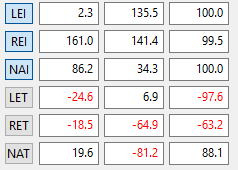
\includegraphics[scale=0.5]{../user_guide_figures/invesalius_screen/nav_selec_coord_en.png}
\caption{Buttons and coordinates to select anatomical fiducials.}
\label{fig:nav_selec_coord}
\end{figure}

The buttons acronyms represent:

\begin{itemize}
	\item LEI: left ear in image
	\item REI: right ear in image
	\item NAI: nasion in image
	\item LET: left ear with spatial tracker
	\item RET: right ear with spatial tracker
	\item NAT: nasion with spatial tracker
\end{itemize}

\begin{figure}[!htb]
\centering
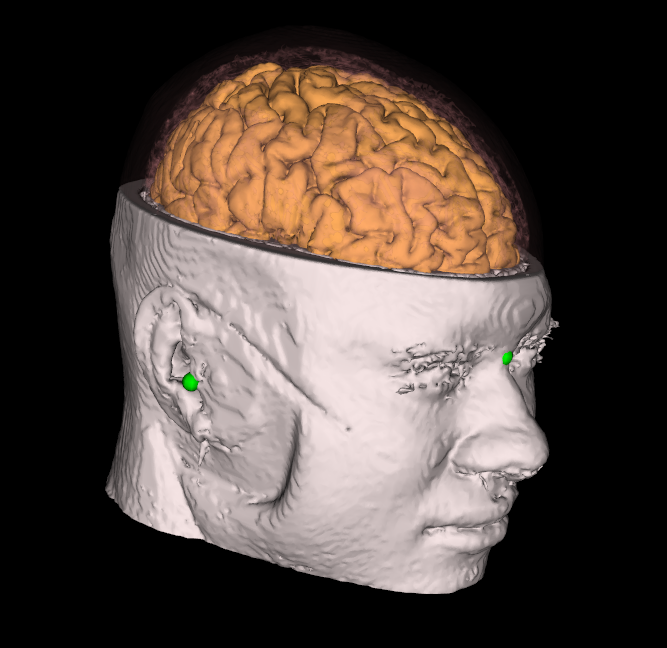
\includegraphics[scale=0.5]{../user_guide_figures/invesalius_screen/nav_balls_in_head.png}
\caption{Selected fiducial markers represented as green spheres.}
\label{fig:nav_balls_in_head}
\end{figure}


\section{Fiducial registration error and navigation}

After all fiducials are selected in both spaces (tracker and image), press the \textbf{Navigate} button to start the neuronavigation process. To stop navigation, simply press \textbf{Navigate} again. Immediately after the navigation starts, the \textbf{Fiducial Registration Error} (FRE) is calculated. The FRE is the root mean square distance between the image fiducials used before and after registration.


To the left of the Navigate button there is a FRE text box. If FRE is high (greater than 3 mm) the navigation will not be precise and the text box will become red (Figure~\ref{fig:nav_fre_error}). If this occurs, the coregistration should be redone. If FRE is lower than 3 mm, the text box will turn green, showing that the navigation has an acceptable precision (Figure~\ref{fig:nav_fre_ok}).

\begin{figure}[!htb]
\centering
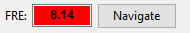
\includegraphics[scale=0.6]{../user_guide_figures/invesalius_screen/nav_fre_error_en.png}
\caption{Navigation button and high FRE unsuitable for navigation.}
\label{fig:nav_fre_error}
\end{figure}

\begin{figure}[!htb]
\centering
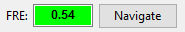
\includegraphics[scale=0.6]{../user_guide_figures/invesalius_screen/nav_fre_ok_en.png}
\caption{Navigation button and low FRE suitable for navigation.}
\label{fig:nav_fre_ok}
\end{figure}

\section{Markers}

During navigation, it is possible to create sphere markers in the 3D space. To do so, select the \textbf{Extra tools} tools tab (Figure~\ref{fig:nav_extra_tools}).

\begin{figure}[!htb]
\centering
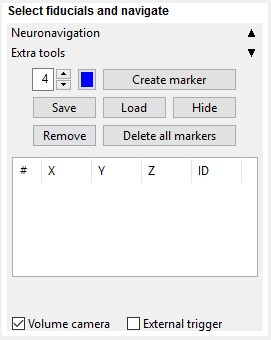
\includegraphics[scale=0.6]{../user_guide_figures/invesalius_screen/nav_extra_tools_en.png}
\caption{Markers manipulation tab.}
\label{fig:nav_extra_tools}
\end{figure}

The marker will be positioned in the current red cross position. The size and color can be changed as needed (Figure~\ref{fig:nav_vol_with_markers}).

When a marker is created, its coordinates will appear in the list control. To identify one marker in the volume, \textbf{double-click with the left} mouse button on the target item and the corresponding marker will blink. To stop blinking, select another marker. It is also possible to create an ID for the marker; simply right click and select \textbf{Edit ID} (Figure~\ref{fig:nav_id_list_markers}). Finally, a window will open allowing the user to define the ID (Figure~\ref{fig:nav_edit_id_markers}).

\begin{figure}[!htb]
\centering
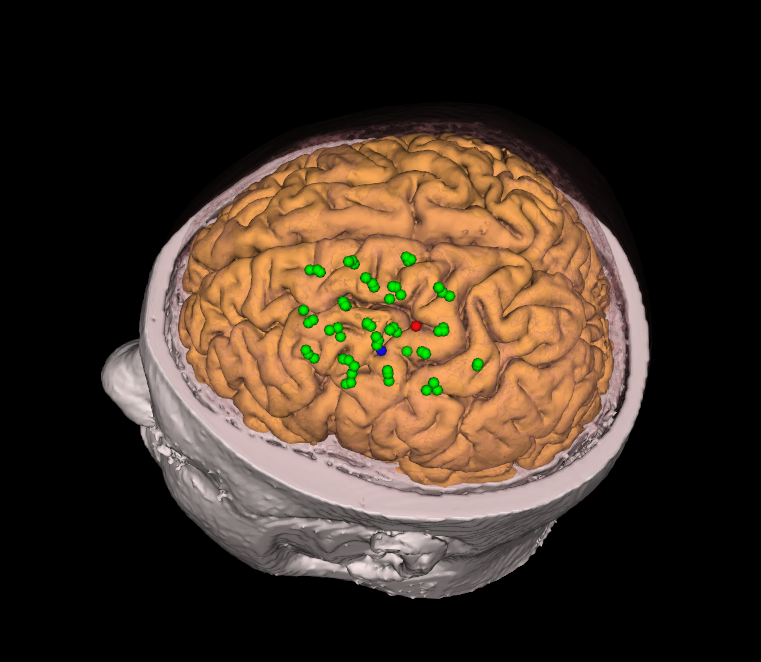
\includegraphics[scale=0.4]{../user_guide_figures/invesalius_screen/nav_vol_with_markers.png}
\caption{Volume with different colors markers.}
\label{fig:nav_vol_with_markers}
\end{figure} 

\begin{figure}[!htb]
\centering
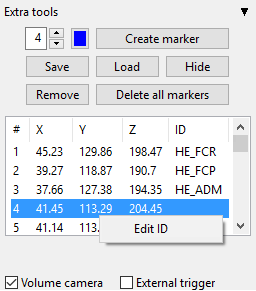
\includegraphics[scale=0.6]{../user_guide_figures/invesalius_screen/nav_id_list_markers_en.png}
\caption{Task to manage marker creation.}
\label{fig:nav_id_list_markers}
\end{figure} 

\begin{figure}[!htb]
\centering
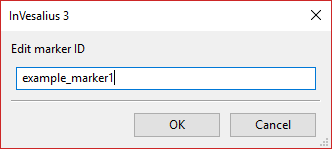
\includegraphics[scale=0.6]{../user_guide_figures/invesalius_screen/nav_edit_id_markers_en.png}
\caption{Window to label the marker.}
\label{fig:nav_edit_id_markers}
\end{figure} 

The marker coordinates may be exported using the \textbf{Save} button (the file extension will be \textit{.mks}). This extension can be opened in any word processor, e.g. Notepad or WordPad software. The file will contain the $X$, $Y$ and $Z$ coordinates followed by the RGB code, marker size and ID. Afterwards, the markers can be imported into the navigation system using the \textbf{Load} button.

To remove markers, \textbf{select} one or more markers needing deletion and press \textbf{Remove}. It is also possible to remove all markers, with the button \textbf{Remove all markers}. All markers can be hidden or shown in the volume using the \textbf{show/hide button}.

\section{External trigger checkbox}

Markers can also be created by using an external trigger. To activate this feature, press the checkbox \textbf{External trigger} before starting navigation. This function was developed to communicate with TMS devices by creating a marker where the pulses are applied, and can be adapted as the user requires. Communication with an external device requires serial port COM1. If this port receives any RS-232 signal at a 9600 \textit{baud rate} it will create a marker in the current red cross position.

\section{Camera volume checkbox}

The volume camera positioning is updated automatically, both by the red cross and the spatial tracker probe position. The user can disable this function by unchecking the \textbf{Camera volume} checkbox. However, the camera has to be manually changed.
